\begin{figure}[h]
    \centering
    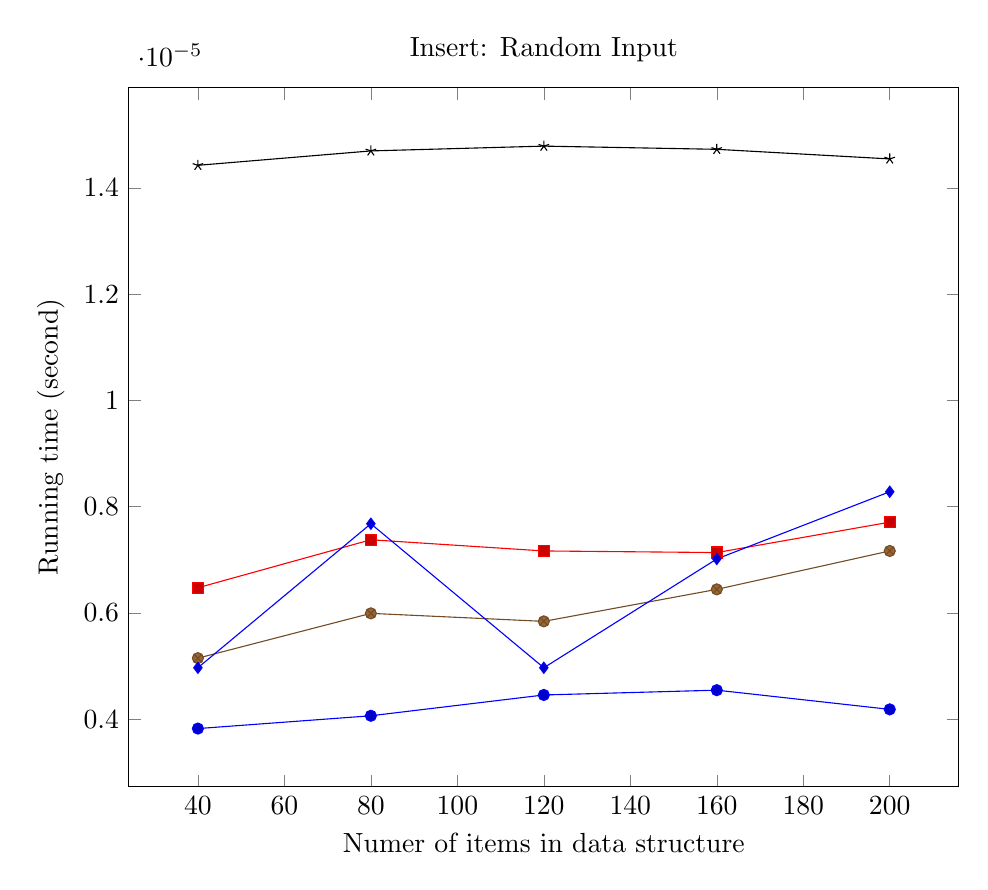
\begin{tikzpicture}
        \begin{axis}[
            xlabel={Numer of items in data structure},
            ylabel={Running time (second)},
            title={Insert: Random Input},
            width=\textwidth
        ]
		\addplot coordinates {
			(40, 3.824926776729854e-06)
			(80, 4.065867046065818e-06)
			(120, 4.4573949839588066e-06)
			(160, 4.54774758509302e-06)
			(200, 4.186337180556166e-06)
		};
		\addplot coordinates {
			(40, 6.475269740136014e-06)
			(80, 7.378795750412337e-06)
			(120, 7.167973014787777e-06)
			(160, 7.1378554810763715e-06)
			(200, 7.710088620882516e-06)
		};
		\addplot coordinates {
			(40, 5.150098258255298e-06)
			(80, 5.993389201464084e-06)
			(120, 5.842801533262332e-06)
			(160, 6.445152206424609e-06)
			(200, 7.167973014787777e-06)
		};
		\addplot coordinates {
			(40, 1.4426298630354495e-05)
			(80, 1.4697356433401865e-05)
			(120, 1.4787709034536078e-05)
			(160, 1.472747396711327e-05)
			(200, 1.4546768765200114e-05)
		};
		\addplot coordinates {
			(40, 4.969393056342142e-06)
			(80, 7.679971087171112e-06)
			(120, 4.969393056342142e-06)
			(160, 7.017385346230754e-06)
			(200, 8.28232176068866e-06)
		};
        \legend{}
        \end{axis}
    \end{tikzpicture}
    \caption{Average of 0 operations, benchmarked every 0, starting at 0.}
\end{figure}